\chapter{TINJAUAN PUSTAKA}
\label{chap:tinjauanpustaka}

\section{Hasil penelitian/perancangan terdahulu}
Pada bagian ini akan dibahas hasil penelitian atau perancangan terdahulu yang relevan dengan penelitian yang akan dilakukan. Penelitian atau perancangan terdahulu tersebut akan dibahas berdasarkan metode yang digunakan, hasil yang diperoleh, dan kesimpulan yang diambil.
\subsection{\emph{Wireless Head Gesture Controlled Wheel Chair for Disable Persons}}
Penelitian yang dilakukan oleh Shayban dan Abdul ini membuat kontrol pergerakan kursi roda dengan menggunakan \emph{accelerometer} yang ditempel diatas topi. \emph{Accelerometer} tersebut dapat mengetahui gestur kepala dari nilai \emph{Axis-X} dan \emph{Axis-Y}.Karena penelitian ini masih mengharuskan penggunanya menggunakan topi yang membuat kontrol pergerakan kursi roda menjadi kurang praktis dan kurang nyaman untuk beberapa pengguna karena ukuran topi yang meskipun bisa di sesuaikan tapi tetap terlalu besar atau terlalu kecil. Jika topinya terlalu besar, maka akan mengganggu akurasi pendeteksian dan jika terlalu kecil, maka pengguna tidak dapat memakainya.

\subsection{Kursi Roda Elektrik dengan Kendali Gestur Kepala}
Penelitian yang dilakukan oleh Tiar, Iyus, dan Trie ini membuat kontrol pergerakan kursi roda dengan menggunakan \emph{accelerometer} dan \emph{ultrasonic}. \emph{Accelerometer} digunakan untuk mengendalikan kursi roda dengan gestur kepala dan \emph{ultrasonic} digunakan untuk melakukan pendeteksian jarak. \emph{Accelerometer} yang digunakan ditempel di kepala pengguna agar dapat melakukan pendeteksian gestur kepala. Penelitian ini mengharuskan penggunanya mengenakan \emph{accelerometer} sehingga dapat membuat penggunanya kurang nyaman.


\section{Dasar Teori}
Pada bagian ini akan dibahas dasar teori yang digunakan dalam penelitian ini. Dasar teori tersebut meliputi teori-teori yang mendukung penelitian ini, seperti teori tentang kursi roda elektrik, DC motor, head gesture, mediapipe, \emph{convolutional neural network} (CNN), \emph{metrics} evaluasi, TensorFlow, Python, kamera, DC-DC voltage regulator, H-bridge motor driver, ESP32 Devkit V1, dan NUC.

\subsection{Kursi Roda Elektrik}
Kursi roda adalah alat yang digunakan untuk meningkatkan kemampuan mobilitas bagi orang yang memiliki kekurangan, seperti orang yang cacat fisik (khususnya penyandang cacat kaki), pasien rumah sakit yang tidak diperbolehkan untuk melakukan banyak aktivitas fisik, orang tua, lanjut usia, dan orang-orang yang memiliki resiko tinggi untuk terluka bila berjalan sendiri \parencite{Ady2011}. Penggunaan kursi roda konvensional cenderung berfokus pada penggunaan manual yang masih mengasumsikan pengguna dapat menggunakan tangan mereka untuk menggerakan kursi roda secara maksimal \parencite{sumit2017}

Secara umum, kursi roda yang digunakan oleh masyarakat dibagi menjadi dua macam, yaitu kursi roda elektrik dan kursi roda manual. Perbedaan dari kedua kursi roda ini terletak pada tenaga penggeraknya. Kursi roda elektrik bergerak dengan tenaga listrik dari baterai dan memiliki beberapa metode untuk mengendalikannya \parencite{Fatoni2023}.

Kursi roda elektrik yang akan digunakan pada penelitian kali ini adalah kursi roda elektrik Onehealth \emph{electric wheelchair}KY-123 yang telah diregistrasikan di Kementerian Kesehatan Republik Indonesia dan memiliki surat izin edar secara resmi. 

\begin{figure} [ht] \centering
    % Nama dari file gambar yang diinputkan
    \includegraphics[scale=0.25]{gambar/Kursi Roda Elektrik Lipat OneHealth KY123 A.jpg}
    % Keterangan gambar yang diinputkan
    \caption{Kursi Roda Elektrik}
    % Label referensi dari gambar yang diinputkan
    \label{fig:Proses Flattening}
\end{figure}

\subsection{DC Motor}
Pada kursi roda elektrik, terdapat dua buah DC motor untuk menggerakkan rodanya. Satu DC motor dipasang di roda kanan dan satunya lagi dipasang di roda kiri.

DC motor adalah sebuah mesin yang mengubah DC daya menjadi tenaga mekanik dikenal dengan istilah DC motor. Pengoperasiannya didasarkan pada prinsip bahwa ketika ada arus yang mengalir konduktor ditempatkan dalam medan magnet, konduktor mengalami mekanik memaksa. Arah gaya ini diberikan oleh aturan tangan kiri Fleming dan besarnya diberikan oleh:


\begin{equation}
    \label{eq:biot-savart}
    F = BI\ell{} 
    \textnormal{ newton}
\end{equation}


Pada dasarnya, tidak ada perbedaan konstruksi antara DC motor dan DC generator. DC yang sama. mesin dapat dijalankan sebagai generator atau motor\parencite{dcmotor}. Pada kursi roda elektrik KY-123, digunakan Motor DC MY1016Z.

\subsection{Head Gesture}
Gestur kepala atau \emph{Head gesture} berarti posisi yang dilakukan oleh pergerakan kepala dengan mempertimbangkan seluruh geometri wajahnya seperti mata, hidung, bibir, dan lain-lain. Kegunaan dari isyarat tersebut adalah untuk mengekspresikan pikiran, emosi, dan lain-lain. Gestur kepala seperti itu sangat berguna dan bermanfaat bagi penyandang cacat atau orang yang mengalami kelumpuhan dari leher dan seterusnya \parencite{bankar}.

\subsection{Mediapipe}
Mediapipe merupakan sebuah framework yang dirancang dengan cara mengimplementasikan kecerdasan buatan kedalam aplikasi yang akan dibangun. Mediapipe tersebut digunakan oleh Google dalam menentukan karakteristik yang ada dalam video. Hal yang dilakukan oleh Google dengan mengumpulkan semua dataset kemudian memberikan label serta mengidentifikasi setiap landmark-nya secara manual. Kecerdasan buatan pada pengaplikasiannya secara garis besar terbagi tujuh cabang, yaitu machine learning, natural language processing, expert system, vision, speech, planning dan robotics. Cabang dari kecerdasan buatan tersebut dimaksudkan untuk ruang lingkup saat pengembangan atau belajar artificial intelligence karena pada dasarnya kecerdasan buatan memiliki ruang lingkup yang sangat luas dan beragam\parencite{MediaPipe2023}.

Pada mediapipe terdapat tiga pendeteksian yang kemudian dapat dibuat lebih spesifik lagi, yaitu head gesture, hand gesture, dan pose detection. Head gesture atau pendeteksian gestur kepala dapat dibuat lebih spesifik menjadi pendeteksian pupil mata dan mulut. Hand gesture atau pendeteksian gesture tangan dapat dibuat lebih spesifik menjadi pendeteksian jari-jemari. Pose detection adalah pendeteksian pose seluruh badan yang dapat dibuat menjadi lebih spesifik seperti pendeteksian gerak kaki atau tangan. Hal yang menarik penulis untuk melakukan penelitian terhadap kecerdasan buatan ini adalah bagian head gesture recognition. Head gesture recognition ini berupa face landmarker yang menggunakan serangkaian model untuk memprediksi landmark wajah. Model pertama mendeteksi wajah, model kedua menemukan penanda pada wajah yang terdeteksi, dan model ketiga menggunakan penanda tersebut untuk mengidentifikasi fitur dan ekspresi wajah. Model berikut dikemas bersama ke dalam bundel model yang dapat diunduh. Pertama, model deteksi wajah yang mendeteksi keberadaan wajah dengan beberapa penanda wajah utama. Kedua, model face mesh yang menambahkan pemetaan wajah secara lengkap. Model tersebut menghasilkan perkiraan 468 landmark wajah 3 dimensi. Ketiga, model prediksi blendshape yang akan menerima keluaran dari model face mesh yang memprediksi 52 skor blendshape, yang merupakan koefisien yang mewakili ekspresi wajah yang berbeda\parencite{MediaPipe2023}.

\begin{figure} [H] \centering
  % Nama dari file gambar yang diinputkan
  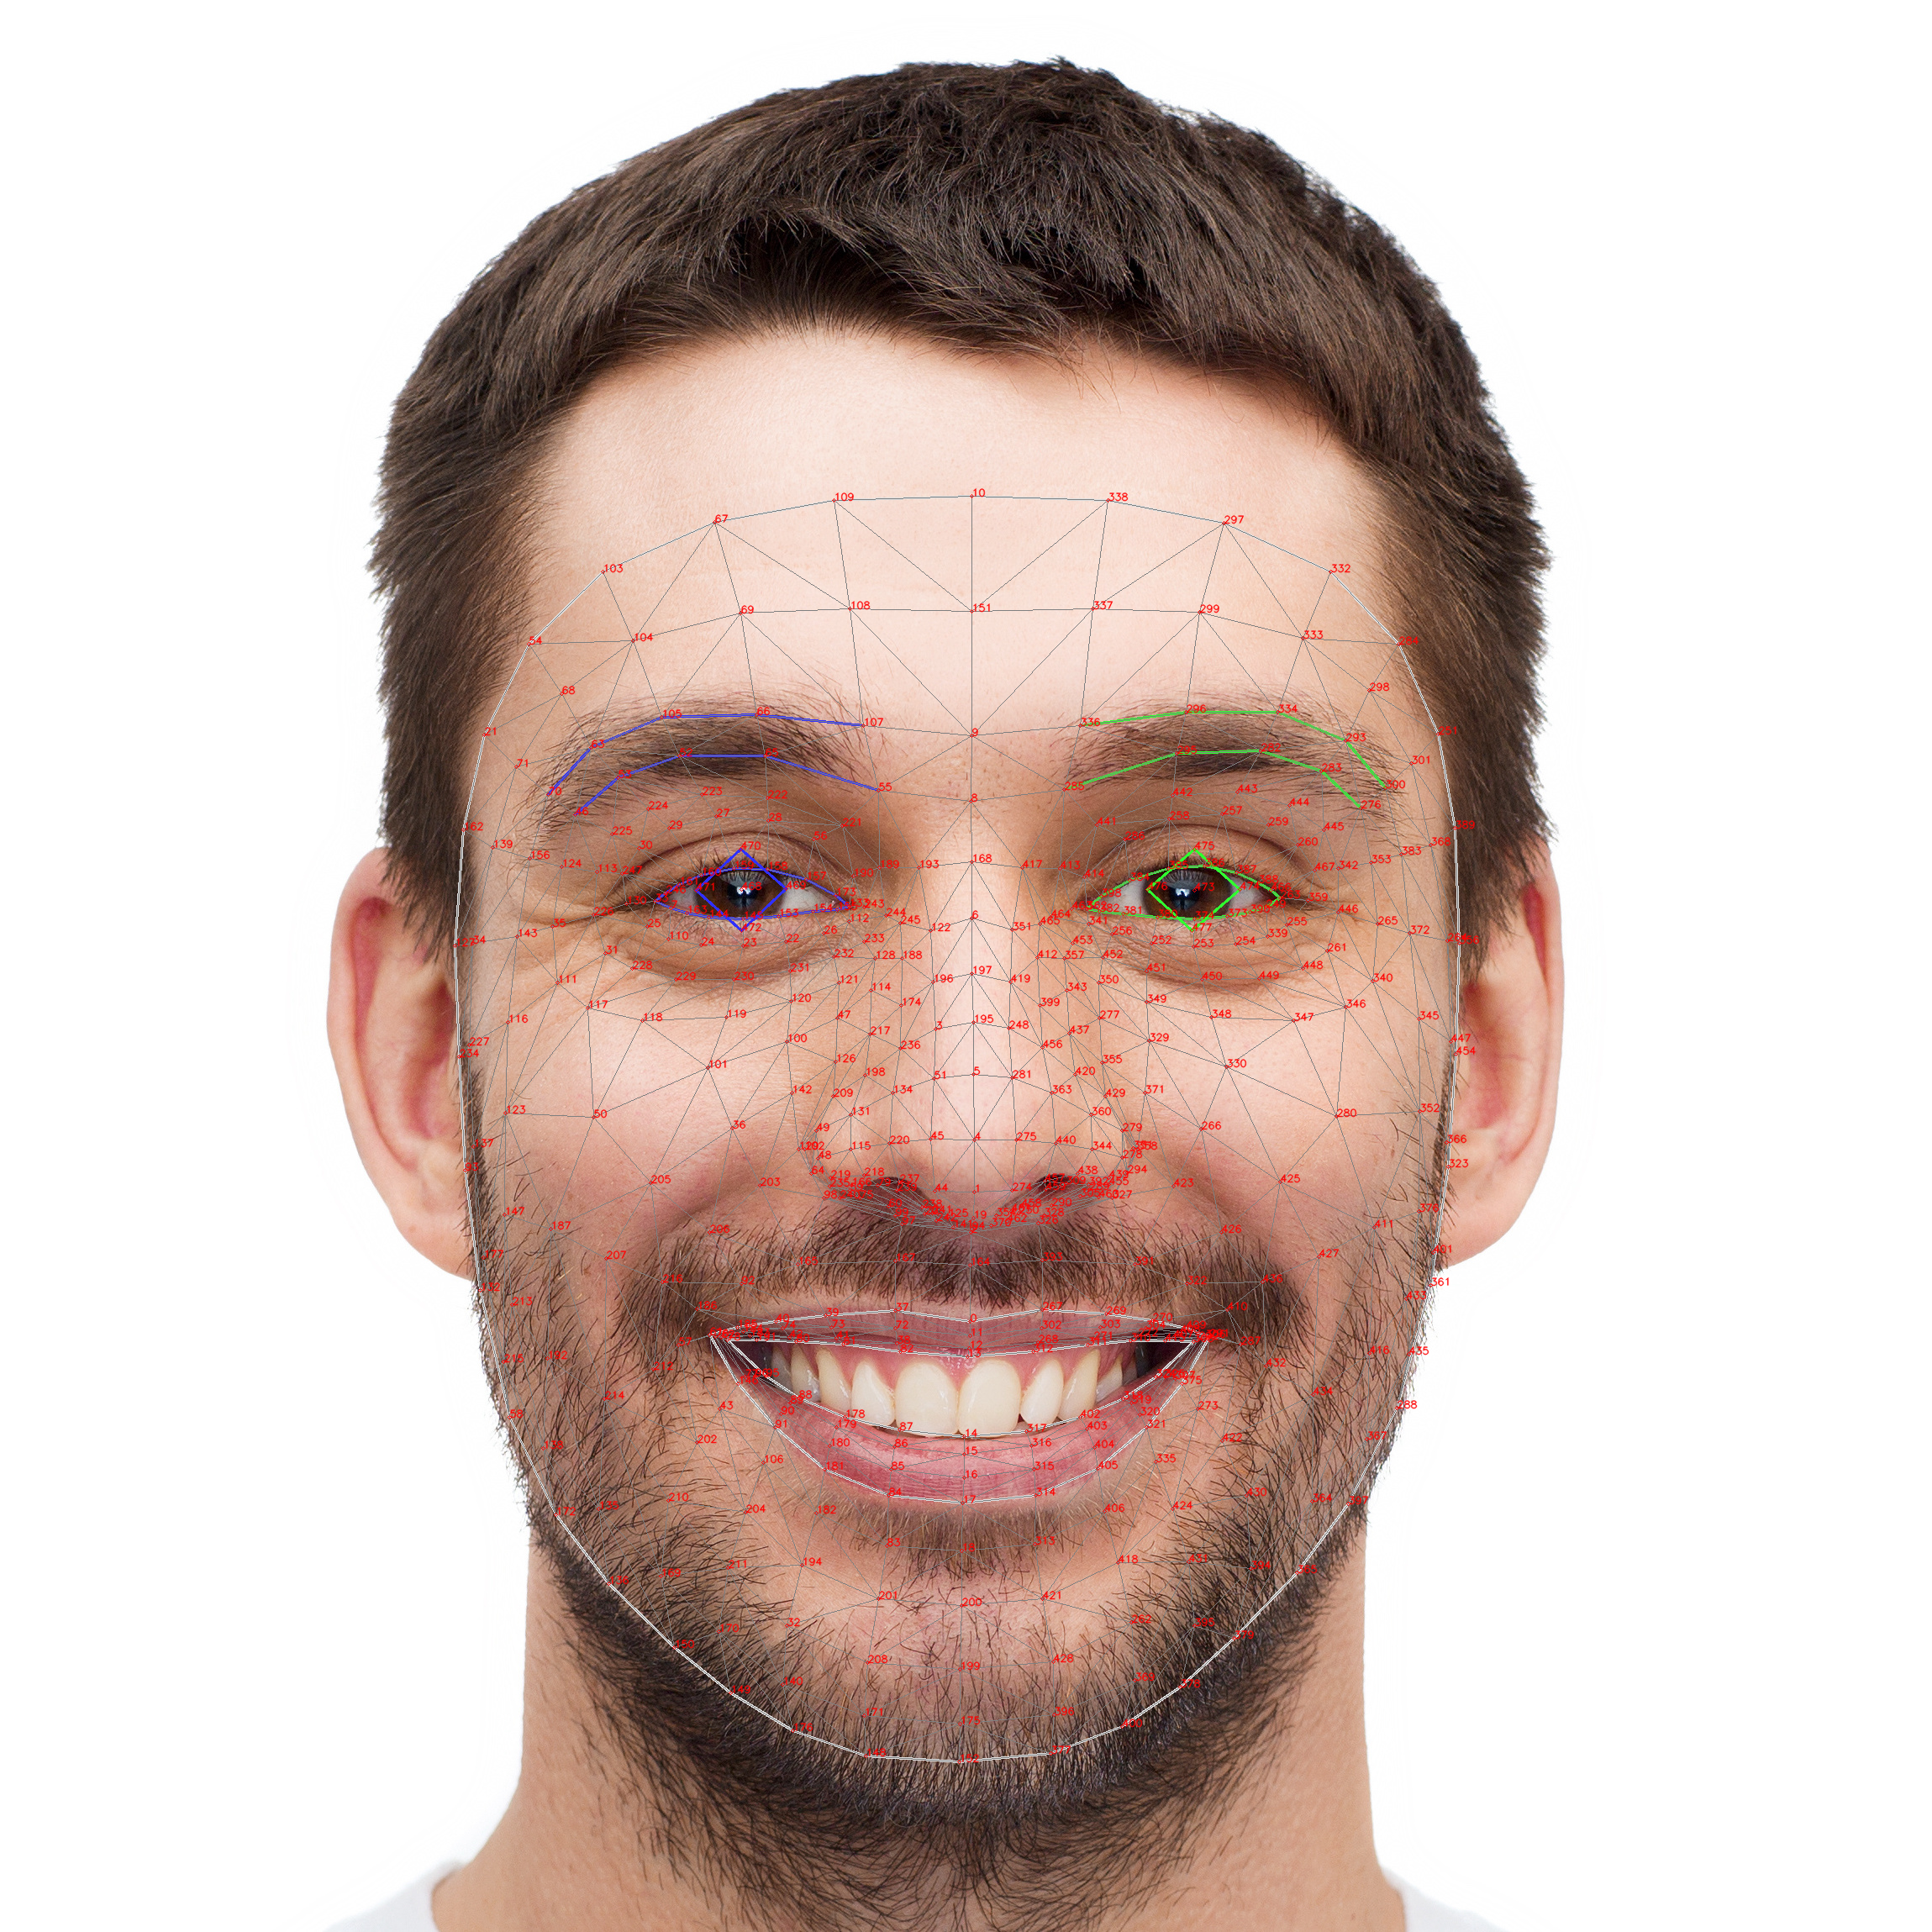
\includegraphics[scale=0.1]{gambar/facelandmark.png}
  % Keterangan gambar yang diinputkan
  \caption{Koordinat \emph{Landmark }}
  % Label referensi dari gambar yang diinputkan
  \label{fig:Blueprint}
\end{figure}

\subsubsection{Citra Wajah}
Pada penelitian ini, citra wajah adalah bahan utama untuk melakukan proses eksplorasi dan ekstraksi data. Citra wajah yang digunakan pada penelitian ini diklasifikasikan menjadi lima kondisi, yaitu hadap depan, hadap kanan, hadap kiri, hadap atas, dan hadap bawah. Citra wajah pada penelitian ini ditangkap oleh kamera yang kemudian akan digambarkan garis-garis landmark dan diubah backgroundnya selain landmark-landmark tersebut menjadi hitam.

\subsection{\emph{Convolutional Neural Network} (CNN)}
\emph{Convolutional Neural Network} (CNN)  telah mencapai hasil yang revolusioner selama dekade terakhir dalam berbagai bidang yang terkait dengan pengenalan pola, mulai dari pemrosesan gambar hingga pengenalan suara. Aspek paling bermanfaat dari CNN adalah mengurangi jumlah parameter dalam \emph{Artificial Neural Network} (ANN). Pencapaian ini telah mendorong para peneliti dan pengembang untuk mengembangkan model yang lebih besar guna menyelesaikan tugas-tugas kompleks, yang tidak mungkin dilakukan dengan ANN klasik. Asumsi penting tentang masalah yang dipecahkan oleh CNN adalah fitur-fitur yang tidak bergantung pada lokasi secara spasial. Sebagai contoh, dalam aplikasi pendeteksian wajah, kita tidak perlu memperhatikan di mana wajah berada dalam gambar. Yang penting adalah mendeteksi mereka tanpa memandang posisi mereka dalam gambar yang diberikan. Aspek penting lain dari CNN adalah untuk memperoleh fitur-fitur abstrak ketika input menyebar menuju lapisan-lapisan yang lebih dalam.\parencite{albawi}.

Arsitektur pada CNN terdiri dari tiga bagian, yaitu input, \emph{feature learning}, dan \emph{classification}. \emph{Feature Learning} terdiri dari dua buah \emph{convolution layer} dan dua buah \emph{pooling layer}. Pada \emph{classification} terdiri dari dua \emph{hidden layer} dan satu \emph{output layer}. Arsitektur CNN dapat digambarkan seperti pada Gambar 2.1.

% Gambar 2.1
\begin{figure} [ht] \centering
    % Nama dari file gambar yang diinputkan
    \includegraphics[scale=0.12]{gambar/arsitekturcnn.png}
    % Keterangan gambar yang diinputkan
    \caption{Arsitektur pada \emph{Convolutional Neural Network}}
    % Label referensi dari gambar yang diinputkan
    \label{fig:arsitektur cnn}
\end{figure}

Input CNN merupakan array tiga dimensi dengan ukuran seperti pada Persamaan \ref{eq:cnn}. Apabila input merupakan suatu citra maka citra tersebut harus diubah menjadi array dua dimensi. 

% Persamaan 2.1
\begin{equation}
  \label{eq:cnn}
Baris * Kolom * Depth
\end{equation}

\emph{Convolution Layer} digunakan untuk menyaring (\emph{filter}) matriks dari citra \emph{input}. \emph{Zero Padd-ing} akan diperlukan untuk mempertahankan ukuran matriks dari citra \parencite{dwitama2019klasifikasi}. Ukuran kernel yang digunakan pada layer konvolusi adalah \(3 \times 3\) dan \(5 \times 5\). \emph{Output} dari lapisan konvolusi ini akan digunakan sebagai \emph{input} pada \emph{Pooling Layer} \parencite{hakim2018}. Apabila output dari \emph{Convolution Layer} bernilai negatif maka akan dilakukan perhitungan tambahan berupa aktifasi ReLU. Fungsi aktivasi ReLU akan nilai matriks yang bernilai negatif menjadi nol. Contoh penerapan dari aktivasi ReLU dapat dilihat pada Gambar \ref{fig:Aktivasi ReLU}.

% Gambar 2.2
\begin{figure} [ht] \centering
    % Nama dari file gambar yang diinputkan
    \includegraphics[scale=1]{gambar/aktivasiReLU.png}
    % Keterangan gambar yang diinputkan
    \caption{\emph{Aktivasi ReLU}}
    % Label referensi dari gambar yang diinputkan
    \label{fig:Aktivasi ReLU}
\end{figure}

\emph{Pooling Layer} digunakan untuk mengurangi jumlah parameter ketika ukuran citra terlalu besar dengan cara mengurangi dimensi setiap fitur. Karena ukuran citra menjadi lebih kecil maka proses \emph{feature map} akan menjadi lebih cepat \parencite{hakim2018}. \emph{Max Pooling} dilakukan dengan cara mengambil nilai dengan elemen terbesar sesuai dengan ukuran filter. Sebagai contoh pada Gambar \ref{fig:Max Pooling} merupakan \emph{max pooling} dengan filter \(2 \times 2\) dengan \emph{stride} sebesar 2.

% Gambar 2.3
\begin{figure} [ht] \centering
    % Nama dari file gambar yang diinputkan
    \includegraphics[scale=1.5]{gambar/maxPooling.png}
    % Keterangan gambar yang diinputkan
    \caption{\emph{Max Pooling}}
    % Label referensi dari gambar yang diinputkan
    \label{fig:Max Pooling}
\end{figure}

Flatten merupakan suatu proses dimana hasil dari \emph{Feature Learning} diubah menjadi vektor yang selanjutnya akan menjadi input pada proses klasifikasi dengan arsitektur \emph{fully connected layer}. Flatten digunakan untuk mengubah matriks menjadi vektor dengan menyesuaikan sesuai format \emph{input} pada \emph{neural network layer}. Flatten dapat digambarkan seperti pada Gambar \ref{fig:Proses Flattening}.

% Gambar 2.4
\begin{figure} [ht] \centering
    % Nama dari file gambar yang diinputkan
    \includegraphics[scale=0.6]{gambar/flattening.png}
    % Keterangan gambar yang diinputkan
    \caption{Proses \emph{Flattening}}
    % Label referensi dari gambar yang diinputkan
    \label{fig:Proses Flattening}
\end{figure}

\subsection{\emph{Metrics} Evaluasi}

Dalam melakukan proses pengklasifikasian, dilakukan evaluasi performa model dengan perhitungan efektifitas model yang telah dibuat. \emph{Confusion Matrix} adalah salah satu perhitungan yang umum digunakan.

Dalam deep learning, evaluasi performa yang sering digunakan adalah \emph{Metrics} tersebut adalah \emph{accuracy, sensitivity (recall), precision} dan \emph{F1-score}. TP, TN, FP, FN adalah parameter yang digunakan dalam pengevaluasian \emph{Metrics} tersebut adalah \emph{accuracy, sensitivity (recall), precision} dan \emph{F1-score}. TP atau \emph{True Positive} adalah jumlah gambar wajah yang teridentifikasi. \emph{True Negative} atau TN adalah jumlah gambar bukan wajah yang terdeteksi. \emph{False Positive} atau FP adalah jumlah salahnya pendeteksian diidentifikasi sebagai wajah yang sebenarnya bukan wajah. \emph{False Negative} atau FN adalah salahnya pendeteksian diidentifikasi sebagai bukan wajah yang sebenarnya adalah wajah \parencite{shajihan}. Visualisasi \emph{confusion matrix} dapat dilihat pada Gambar \ref{fig:confusion}.

% Gambar 2.7
\begin{figure} [ht] \centering
    % Nama dari file gambar yang diinputkan
    \includegraphics[width=.5\textwidth]{gambar/confusionmatrix.png}
    % Keterangan gambar yang diinputkan
    \caption{Visualisasi \emph{confusion matrix}}
    % Label referensi dari gambar yang diinputkan
    \label{fig:confusion}
\end{figure}

\subsubsection{\emph{Accuracy}}
\label{subsec:acc_klasifikasi}

\emph{Accuracy} didefinisikan sebagai rasio benarnya klasifikasi data dengan total jumlah data yang ada\parencite{Ovalle}. Nilai \emph{accuracy} dapat diperoleh menggunakan Persamaan \ref{eq:acc}. 

\begin{equation}
  \label{eq:acc}
  Accuracy=\frac{TP+TN}{TP+TN+FP+FN}
\end{equation}

\subsubsection{\emph{Precision}}
\label{subsec:prec_klasifikasi}

\emph{Precision} (PC) atau nilai prediksi positif, mengukur bagian dari data positif yang diklasifikasikan secara benar\parencite{Ovalle}. Nilai \emph{precision} dapat diperoleh dengan Persamaan \ref{eq:prec}.

\begin{equation}
  \label{eq:prec}
  Precision=\frac{TP}{TP+FP}
\end{equation}

\subsubsection{\emph{Sensitivity}}
\label{subsec:sensitivity_klasifikasi}

\emph{Sensitivity} (SN) yang juga dikenal sebagai tingkat \emph{true positive} atau \emph{recall}, mengukur bagian dari klasifikasi data positif yang benar\parencite{Ovalle}. Dengan demikian, nilai recall dapat dihitung menggunakan Persamaan \ref{eq:recall}.

\begin{equation}
  \label{eq:recall}
  Recall=\frac{TP}{TP+FN}
\end{equation}

\subsubsection{\emph{F-Score}}
\label{subsec:score_klasifikasi}

\emph{Metric F-Score} yang umum adalah dengan menggabungkan perhitungan \emph{precision} dan \emph{recall}. Secara khusus, \emph{F-Score} yang seimbang didapatkan ketika \(\beta\) = 1, oleh karena itu lebih dikenal sebagai perhitungan \emph{F1} \parencite{Ovalle}. Nilai \emph{F1-Score} dapat dihitung menggunakan Persamaan \ref{eq:score}.

\begin{equation}
  \label{eq:score}
  F{1}{-}Score=\frac{2 \times Precision \times Recall}{Precision+Recall}
\end{equation}

\subsection{Tensorflow}
TensorFlow merupakan platform untuk machine learning. TensorFlow memiliki fitur untuk menjalankan training model menggunakan Central Processing Unit (CPU) dan training model Graphic Processing Unit (GPU) yang memiliki waktu training yang lebih cepat dibanding training model CPU \parencite{nurfita2018}.

TensorFlow awalnya dikembangkan oleh para peneliti dan pengembang yang bekerja sebagai tim di Google Brain untuk melakukan penelitian di bidang machine learning dan neural network. Framework ini dirilis pertama kali pada bulan Februari 2017 dan terus dikembangkan hingga sekarang \parencite{Developers}.

\subsection{Python}
Python adalah bahasa pemrograman interpretatif berorientasi objek. Python menawarkan struktur data tingkat tinggi termasuk kamus, modul, kelas, pengecualian, daftar dan array asosiatif, pengetikan dinamis, pengikatan dinamis, dan manajemen memori pintar. Meskipun memiliki sintaks yang sangat mudah dimengerti dan bersih, Python adalah bahasa pemrograman yang kuat dan serbaguna. Python diciptakan pada tahun 1990 oleh Guido van Rossum. Python dapat digunakan dengan bebas, bahkan untuk tujuan komersial, seperti banyak bahasa pemrograman lainnya, dan dapat dieksekusi di hampir semua komputer modern. Interpreter secara otomatis mengubah program Python menjadi kode byte yang tidak tergantung pada platform tempat kode tersebut dijalankan \parencite{Sanner1999Python}.

Python merupakan bahasa pemrograman yang sangat fleksibel, serbaguna, dan dapat digunakan untuk berbagai keperluan seperti skrip, pengembangan aplikasi web, dan lain-lain. Python juga bisa diperkaya dengan bahasa C dan C++, memberikan keunggulan kecepatan untuk tugas-tugas yang memerlukan banyak pemrosesan. Python memiliki struktur yang terorganisir dengan baik, termasuk blok kode yang terstruktur, fungsi, kelas, modul, dan paket, serta konsistensi dalam penggunaan objek dan paradigma pemrograman berorientasi objek. Ini memudahkan dalam mengembangkan aplikasi yang efisien dan mudah dipahami, baik untuk tugas kecil maupun besar. Python dilengkapi dengan berbagai tipe data bawaan yang kompleks seperti string, list, dan dictionary, serta kontrol alur standar seperti if, if-else, while, dan for. Bahasa ini secara otomatis mengompilasi kode sumber menjadi byte code, mendukung ekstensi dalam C dan C++, dan menggunakan indentasi untuk menandai blok kode. Indentasi yang standar adalah empat spasi per tingkat tanpa menggunakan tab, yang memudahkan integrasi kode Python dengan kode dari bahasa lain.


\subsection{Kamera}
Kata “kamera” adalah kependekan dari "kamera obscura", yang merupakan tenda kedap cahaya, memungkinkan proyeksi gambar melalui lubang kecil dengan lensa. Lensa digunakan untuk mengumpulkan dan menyatukan cahaya ke suatu titik, seperti yang terjadi pada cermin pembesar. Seniman yang duduk di dalam ruangan biasa menjiplak gambar yang dibuat pada permukaan datar. Permukaan datar ini kemudian digantikan oleh film fotografi dengan bahan kimia peka cahaya, yang memungkinkan terjadinya reaksi kimia tertentu, yang dipicu oleh cahaya. Basis bahan ini dimulai dengan lembaran kaca lebar dan berkembang menjadi film kecil berukuran 35 mm, sehingga mengurangi ukurannya dan juga meningkatkan kemudahan penggunaan.

Saat ini, dengan kemajuan teknologi digital, fotografi juga telah berkembang pesat selama tiga dekade terakhir. Kamera digital menggunakan prinsip optik yang sama dengan kamera film, dibantu oleh sensor digital yang menggantikan film. Jadi saat sensor menangkap sinyal cahaya, chip lain, atau kartu memori, menyimpan sinyal tersebut dalam bentuk data digital. Data ini kemudian dapat diedit di komputer, ponsel, dll., dan dibagikan melalui Internet ke media sosial, dan juga dapat dicetak dan ditempel di album foto \parencite{inbook}

Kamera webcam yang digunakan adalah logitech C920. Berikut adalah spesifikasi kamera yang digunakan:
\begin{table}[H]
\centering
\begin{tabular}{|l|l|}
\hline
\multicolumn{2}{|c|}{\textbf{Spesifikasi}} \\ \hline
Max Resolution & 1080p/30 fps - 720p/30 fps \\ \hline
Camera Mega Pixel & 3 \\ \hline
Focus Type & Auto Focus \\ \hline
\end{tabular}
\caption{Spesifikasi \emph{Webcam}}
\label{tab:my_label}
\end{table}

\subsection{DC-DC Voltage Regulator}
Regulator/konverter dc-dc atau nama lain yang dikenal dengan buck atau \emph{boost regulator}, memberikan tegangan keluaran yang diatur secara stabil untuk mensuplai rangkaian listrik dan elektronik.

Konverter daya DC-DC digunakan dalam berbagai aplikasi, termasuk catu daya komputer pribadi, peralatan kantor, sistem tenaga pesawat ruang angkasa, komputer laptop, dan peralatan telekomunikasi, serta penggerak motor DC. Masukan ke konverter dc-dc tidak diatur
tegangan DC Vg. Konverter menghasilkan tegangan keluaran yang diatur V, memiliki besarnya (dan mungkin polaritas) itu berbeda dengan Vg\parencite{dcdc}.

\subsection{H-Bridge Motor Driver}
H-bridge adalah sirkuit sederhana yang terdiri dari empat transistor, yaitu dua N-type dan 2 P-type. Transistor P-type terhubung di sisi \emph{high} motor (bagian yang terhubung ke daya) dan transistor N-type ke sisi \emph{low} motor (bagian yang terhubung ke \emph{ground}). Setiap sisi motor terhubung ke amplifier \emph{push-pull} sederhana yang setiap amplifiernya terhubung ke saklar \parencite{hbridge}.
\begin{figure} [H] \centering
    % Nama dari file gambar yang diinputkan
    \includegraphics[scale=0.2]{gambar/hbridge.jpeg}
    % Keterangan gambar yang diinputkan
    \caption{H-Bridge Motor Driver}
    % Label referensi dari gambar yang diinputkan
    \label{fig:hbridge}
\end{figure}


\subsection{ESP32 Devkit V1}
ESP32 Devkit V1 adalah mikrokontroller yang dikembangkan oleh Espressif Systems. ESP32 dirancang berdasarkan arsitektur Xtensa dual-core 32-bit. Hal ini berarti ESP32 memiliki dua buah inti prosesor yang dapat beroperasi secara independen. Salah satu fitur ESP32 yang paling penting adalah WiFi dan Bluetooth yang sudah terintegrasi sehingga memungkinkan ESP32 untuk berkomunikasi dengan perangkat lain secara mudah \parencite{esp32}.
\begin{figure} [H] \centering
    % Nama dari file gambar yang diinputkan
    \includegraphics[scale=0.3]{gambar/esp32 pinout.jpg}
    % Keterangan gambar yang diinputkan
    \caption{ESP32}
    % Label referensi dari gambar yang diinputkan
    \label{fig:Proses Flattening}
\end{figure}

\subsection{NUC}
NUC, yang merupakan singkatan dari “Next Unit of Computing”, adalah komputer berbentuk kotak kecil yang dikembangkan oleh Intel1. Meskipun ukurannya hanya beberapa inci atau lebih dalam, NUC berisi seluruh sistem yang dijejalkan ke dalam chassis kecilnya1. NUC juga bisa dijual sebagai kit barebone yang perlu dirakit oleh pengguna untuk membuatnya bekerja\parencite{nuc}.

Intel NUC memiliki motherboard yang hanya berukuran 4 × 4 inci (10.16 × 10.16 cm)1. Ada banyak pilihan tipe prosesor untuk NUC ini seperti Celeron, Pentium, Core i3, Core i7, hingga Core i92. Intel NUC juga menawarkan solusi Modular Computing dimana komponennya dapat dikostumisasi sesuai dengan kebutuhan2. NUC yang digunakan pada penelitian ini adalah NUC dengan seri NUC11PAHi7. 
\begin{figure} [H] \centering
    % Nama dari file gambar yang diinputkan
    \includegraphics[scale=0.4]{gambar/nuc.png}
    % Keterangan gambar yang diinputkan
    \caption{NUC}
    % Label referensi dari gambar yang diinputkan
    \label{fig:Proses Flattening}
\end{figure}


\subsection{Arduino IDE}
Arduino IDE adalah perangkat lunak sumber terbuka yang dirancang oleh Arduino.cc dan digunakan terutama untuk menulis, mengkompilasi, dan mengunggah kode ke hampir semua Modul Arduino. Ini adalah perangkat lunak Arduino resmi, yang membuat kompilasi kode sangat mudah sehingga bahkan orang biasa tanpa pengetahuan teknis sebelumnya dapat memulai proses pembelajaran. Arduino IDE berjalan pada Platform Java dan dilengkapi dengan fungsi dan perintah bawaan yang memainkan peran penting dalam debugging, pengeditan, dan kompilasi kode \parencite{Watson_2023}.
